% !TEX root=/home/tavant/these/manuscript/src/manuscript.tex




\chapter{Azimuthal instability}
\label{ch-3}

The presence of azimuthal instabilities in the Hall effect thrusters has first been showed with numerical simulations by \citet{adam2004}.
However, it nature is not yet fully understood.
In this chapter, we investigate the instabilities observed in the \ac{2D} \ac{PIC} simulations.

First, we derive the dispersion relation without hypothesis on the particle distribution function.
Then, we present a numerical algorithm that solves the dispersion relation using the distribution function measured in the \ac{PIC} simulations.
Then, the oscillations observed in the simulation are compared to the results of the dispersion relation.

% 
% 
% {\bf V. analyse of the instability } 30 pages
% \begin{zzz}
%   \begin{itemize}
% \item Instability dispersion relation
% \item Kinetic solver for Ion and ECDI using VDFs
% \item Impact of the difference w/r Maxwellian
% \item Wall Boundary condition, 3D dispertion relation vs 1D and 2D relations
% \item Linear stage as ECDI and Saturation toward IAW
% \end{itemize}
% \end{zzz}

\minitoc


% !TEX root=/home/tavant/these/manuscript/src/manuscript.tex

\section{Dispersion relation of the instabilities}
  \label{sec-DR-kinetic}
  
  
  The dispersion relations are obtained by coupling the particle dynamics with the electric fields.
  In the case of the kinetic electrostatic dispersion relation, we couple the Vlasov equation with the Poisson equation.
  In our \ac{2D} geometry, we can neglect all the gradients.
  A fixed axial electric field $\vect{E} = E_0 \vect{e_z}$ and a fixed radial magnetic field $\vect{B} = B_0 \vect{e_r}$ are imposed.
  The electrons are drifting in the azimuthal direction due to the $E\times B$ drift, hence
  \[ \vect{u_{e}} = \frac{\vect{E} \times \vect{B}}{\norm{\vect{B}}^2} = \frac{E_0}{B_0}  \vect{e_{\theta}}.    \]
  The ions are accelerated in the axial direction, $ \vect{u_i} = u_i  \vect{e_z}$.
  Using a perturbations as waves of the form \[ \exp \lp i \vect{k} \cdot \vect{x} - i \omega t  \rp, \]
  with $\vect{x}$ the position vector.
  The oscillation wave vector $\vect{k} = k_r \vect{e_r} + k_{\theta} \vect{e_{\theta}}$ is real but its frequency $\omega = \omega_r + i \gamma$ can be complex, where $\gamma$ is the growth rate of the oscillations. 
  
  \vspace{1em}
  The dispersion relation has been studied by \citet{ducrocq2006} in the case of cold ions and Maxwellian electrons in a \ac{2D} geometry.
  A numerical algorithm has been proposed by \citet{cavalier2013} and compared to experimental measurements.
  In \citet{lafleur2016}, the authors added the ion drift velocity to the dispersion relation.
  
  The \ac{ECDI} dispersion relation obtained presents resonances at the cyclotron frequencies, which broadens when $k_r$ increased.
  The limit when $k_r$ tends to large values is similar to an \ac{IAW}.
  This limit is usually used, even if recently, \ac{2D} \ac{PIC} simulations with a larger domain observed radial structures in the oscillations \citep{janhunen2018,hara2019a}.
  
  \citet{lafleur2018} removed the Maxwellian hypothesis by using directly the distribution functions measured in the \ac{PIC} simulations in the \ac{IAW} dispersion relation.
  The authors showed that the frequency of the oscillation is almost unperturbed, but the growth rate is significantly reduced, even when the ions were still supposed Maxwellian \citep[Fig. 8]{lafleur2018}.
  
  Here, we propose to continue the investigation by solving the dispersion relation numerically with the electron and ion distribution function for both the \ac{IAW} and the \ac{ECDI}.
  
  
  \subsection{General dispersion relation}
    \label{sec-geneDR}
    
    We follow the development presented in \citet{ducrocq2006,cavalier2013,lafleur2016}.
    The plasma dielectric function is defined as
    \begin{equation} \label{eq-de}
      \hat\epsilon(\vect{k},\omega) = 1 - \sum_s \chi_s(\vect{k},\omega)
    \end{equation}
    
    where $\chi_s(\vect{k}, \omega)$ is the susceptibility of the species $s$.
    It is obtained by coupling the Poisson equation with the particles description.
    The dispersion relation is obtained by setting $  \hat\epsilon(\vect{k},\omega) =0$ and solving for $\vect{k},\omega$.
    
    
    For the unmagnetized ions, supposing a Maxwellian distribution, the susceptibility is
    \begin{equation} \label{eq-susceptibility}
      \chi_i(\vect{k},\omega) = \frac{\opi^2}{k^2 v^2_{th, i}} Z'\lp \frac{\omega - \vect{k} \cdot \vect{u_{i}}}{k v_{th, i}}  \rp
    \end{equation}
    where $\opi$ the ion plasma pulsation, $k=\norm{\vect{k}}$ and $\vect{u_i}$ is the mean velocity of the ions.
    The function $Z'$ is the derivative of the Fried and Conte function \citep{fried1961}
    \begin{equation} \label{eq-friedandConte}
      Z(\eta) = \frac{1}{\sqrt{\pi}} \int_{-\infty}^{\infty} \frac{\exp{(-t^2)}}{t - \eta} dt.
    \end{equation}
    We use here the Fried and Conte function because of the Maxwellian hypothesis.
    \citet{xie2013} proposes a numerical algorithm to calculate the susceptibility for a general distribution function
    \begin{equation} \label{eq-general}
      Z(\eta, f) = \int_{-\infty}^{\infty} \frac{f(t)}{t - \eta} dt,
    \end{equation}
    with $f$ the velocity distribution function to consider, normalized to one, centered, and of standard deviation $\sigma = 1/2$.
    For the sake of brevity, the generalized dispersion function $Z(\eta,f)$ is noted $Z(\eta)$, and the Fried and Conte function is noted $Z_M(\eta)$.
    The derivative of $Z$ is
    \begin{equation} \label{eq-derivatives}
      Z'(\eta) = \int_{-\infty}^{\infty} \frac{\partial f(t) / \partial t}{t - \eta} dt,
    \end{equation}
    
    \vspace{1em}
    A general expression for the plasma dielectric function can be obtained for magnetized electrons by making use of the method of characteristics and is given by
    \begin{equation} \label{eq-drECDI}
      \begin{split}
      \hat\epsilon(\vect{k},\omega) =& 1 - \\
       &\frac{\opi^2}{k^2 v^2_{th, i}} Z'\lp \frac{\omega - \vect{k} \cdot \vect{u_{i}}}{k v_{th, i}}  \rp + \\
       & \frac{1}{k^2 \lde^2} \lb 1 + \lp  \frac{\omega - \vect{k} \cdot \vect{u_{e}}}{k v_{th, e}} \rp \sum_{n=-\infty}^{\infty} e^{- \beta} I_n(\beta) Z\lp  \frac{\omega - \vect{k} \cdot \vect{u_{e} - n \oce}}{k_{r} v_{th, e}} \rp  \rb,
    \end{split}
    \end{equation}
    where $I_n$ are the modified Bessel functions of the first kind, and 
    \begin{equation} \label{eq-beta}
      \beta = \frac{(k_{\theta}^2 + k_z^2) b^2_{th, e}}{ \oce^2}
    \end{equation}
    
    \Cref{eq-drECDI} is the dispersion relation for drifting magnetized electrons and unmagnetized ions.
    It will be used to study the \acf{ECDI}.
    


  \subsection{Modified Ion Acoustic Wave}
    \label{sucsec-IAW}
    
    The dispersion relation of \cref{eq-drECDI} presents sharp resonances due to cyclotron resonances.
    However, kinetic simulations in \citet{janhunen2018} and \citet{taccogna2019} have shown that after some time (around  $t=0.5\,\micro\second$ and $t=3\,\micro\second$ respectively) the resonances are no longer present, with a progressive decrease of the higher harmonics and the first harmonics becoming the most prominent.
    Without the resonances, the dispersion relation evolves to the nonmagnetic ion-acoustic instability
    \begin{equation} \label{eq-drIAWgene}
      \begin{split}
      \hat\epsilon(\vect{k},\omega) =& 1 - \\
       &\frac{\opi^2}{k^2 v^2_{th, i}} Z'\lp \frac{\omega - \vect{k} \cdot \vect{u_{i}}}{k v_{th, i}}  \rp + \\
       & \frac{1}{k^2 \lde^2}  Z'\lp  \frac{\omega - \vect{k} \cdot \vect{u_{e}}}{k v_{th, e}} \rp ,
    \end{split}
    \end{equation}

    \citet{lafleur2016} and \citet{janhunen2018} show that after some assumptions -- mostly a drifting Maxwellian distribution, cold ions, and a small electron drift velocity compared to thermal speed -- \cref{eq-drIAWgene} can be solved to obtain
    \begin{equation} \label{eq-MIAW}
      \omega = \omega_r + i \gamma = \vect{k} \cdot \vect{u_{i}} \pm \frac{k c_s}{\sqrt{1 + k^2 \lde^2}} \pm i \sqrt{\frac{\pi m_e}{8 m_i}} \frac{\vect{k} \cdot \vect{u_{e}}}{( 1 + k^2 \lde^2)^{3/2}}.
    \end{equation}
    The above equation represents the analytic modified ion-acoustic dispersion relation.
    The wavenumber that corresponds to the maximum growth rate is \citep{lafleur2016}
    \begin{equation} \label{eq-mostk}
      k_{max} = \frac{1}{\sqrt{2} \lde}
    \end{equation}
    which gives, subtituted in \cref{eq-MIAW}
    \begin{equation} \label{eq-mostw}
      \omega_{max} =  \vect{k} \cdot \vect{u_{i}} \pm \frac{\opi}{\sqrt{3}} + i \sqrt{ \frac{\pi m_e}{54 m_i}}\frac{u_e}{\lde}
    \end{equation}
    We can see that the growth rate is proportional to the electron drift velocity, and inversely proportional to the Debye length.
    
    However, one should note that there is no consensus on the transition to an \ac{IAW}.
    It could be attributed to non-linear resonance broadening, because the electron orbit is distorted, leading to the loss of the phase relation between the electron and the wave \citep{taccogna2019}.
    The electron demagnetization leads to a dispersion relation where the ions and the electrons have the same type of contribution.
    But recently, \citet{janhunen2018a} stated that the demagnetization condition due to nonlinear resonance broadening is not fulfilled.
    \citet{lafleur2017a} uses the fact that in \ac{2D} simulations, the finite minimum value for the radial wave vector is responsible for the ion acoustic dispersion relation.
    
    
% !TEX root=/home/tavant/these/manuscript/src/manuscript.tex

\section{Solving the kinetic \acs{DR} for general distribution functions}
  \label{sec-DR-solver}
  \renewcommand\rightmark{\expandafter\MakeUppercase{Solver for the general DR}}


  In order to solve the dispersion relation $\hat\epsilon(\vect{k}, \omega) = 0$ of \cref{eq-drECDI}, we solve for every $\vect{k}$ the complex value of $\omega$ that minimise $\norm{\hat\epsilon}$.
  Hence, we first need to evaluate $\hat\epsilon(\vect{k}, \omega)$ for given arguments $\vect{k}, \omega$.
  Then, we can find the root.
  
  \subsection{Numerical determination of $\hat\epsilon$} \label{subsec-numepsilon}
  
  The calculation of $Z$, needed to determine $\hat{\epsilon}$, is usually done using the Maxwellian hypothesis \citep{cavalier2013} (hence using the Fried and Compte function $Z_M$), the kappa distribution \citep{ziebell2017}, or other analytic expressions.
  We can also use a linear combination of such simple distribution functions, such as done in the software WHAMP, \citet{ronnmark1982}.
  Here we propose to solve the dispersion relation $\hat{\epsilon}=0$ using the distribution function measured in the \ac{PIC} simulation.
  
  
  The numerical computation of $\norm{\hat\epsilon}$ is done using the method of \citet{xie2013} for computing $\tilde{Z}$ the numerical approximation of $Z$. 
  It uses the fact that $Z$ is an Hilbert transform of the distribution function, and that the Hilbert transform can be changed to a Fourier Transform, weighted by well chosen basis functions, so the \ac{FFT} algorithm can be used \citep{weideman1995}.
  
  An interesting point is that the evaluation of $\tilde{Z}(\eta)$ is done by a polynomial function, which coefficients depends only on the distribution function $f$. 
  Hence, they need to be determined only once, and evaluating $\tilde{Z}(\eta)$ is relatively fast.
  
  \begin{figure}[!hbt]
    \centering
    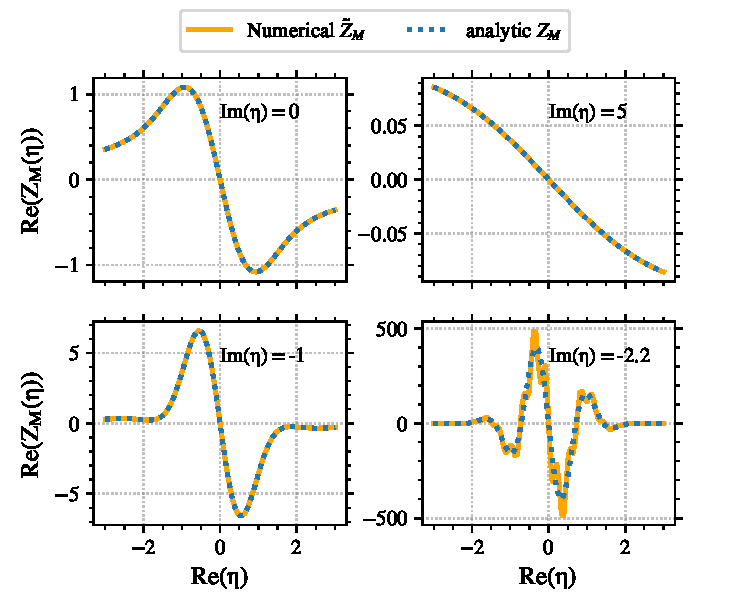
\includegraphics[width=0.8\textwidth]{Validation_numericalZ.pdf}
    \caption{Comparison of the numerical evaluation of $\tilde{Z}_M(\eta)$ for a Maxwellian distribution function with the Fried and Conte function (from the \texttt{plasmapy} python package) for different values of the imaginary part of $\eta: 5, 0,-1,$ and $-2.2$.  }
    \label{fig-numZ}
  \end{figure}
  \cref{fig-numZ} shows the comparison of the numerical evaluation of $\tilde{Z}(\eta)$ for a Maxwellian distribution function with the Fried and Conte function (from the `plasmapy` python package) for different values of the imaginary part of $\eta$.
  We can see that for $\Im(\eta)$ positive, null or slightly negative, the two functions gives exactly the same results.
  However, for larger negative values of $\Im(\eta)$, the two functions gives different results.
  
  This discrepancy between $Z_M$ and $\tilde{Z}_M$ for large negative imaginary argument is certainly due to the fact of the analytic expansion of $Z$ to the complex plane require the evaluation of the distribution function for complex velocities \citep{xie2013,weideman1995}.
  However, the discrete velocity distribution function measured in the \ac{PIC} simulation cannot be properly evaluated for complex velocities.
  On the other hand, we are only interested in instabilities, with positive growth rate.
  Hence, the discrepancy observed should not affect the conclusions of the study.
  


  \begin{figure}[hbt]
    \centering
    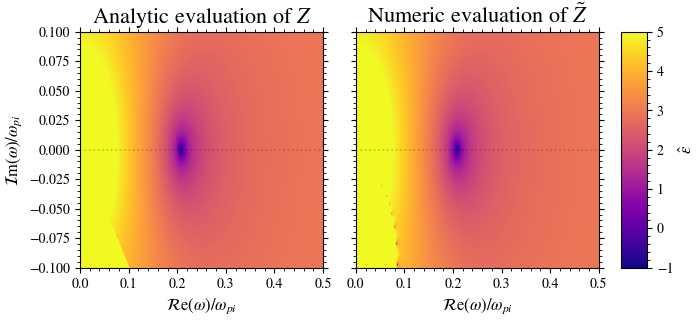
\includegraphics[width=0.8\textwidth]{Validation_numericalZ_bis.png}
    \caption{Comparison of the numerical evaluation of $\hat\epsilon$ from \cref{eq-drECDI} for a Maxwellian distribution function with (left) the Fried and Conte function (from the \texttt{plasmapy} python package) and (right) the numerical $\tilde{Z}$, in logarithmic scale.  }
    \label{fig-numZbis}
  \end{figure}
  
  \Cref{fig-numZbis} presents the comparison of the calculation of $\hat\epsilon$ from \cref{eq-drECDI} for a Maxwellian distribution function with (left) the Fried and Conte function (from the `plasmapy` python package) and (right) the numerical $\tilde{Z}$.
  We can see that the root with the greater imaginary part, located close to (0.2, 0), is the same in both cases, but that other roots for large negative imaginary part are not similar.
  But as said previously, theses roots are not our concern, hence the dispersion relation should be well computed using $\tilde{Z}$.
  
  \subsection{Finding the root of $\hat\epsilon$}
  Now that we can compute $\hat\epsilon$, we can solve the dispersion relation.
  In order to find the root (the zeros) of $\hat\epsilon$, two methods have been tested.
  
  
  \paragraph{Exact root finding algorithm\\}
    The first approach has the advantage of finding all of the roots in a given domain.
    It uses Cauchy's argument principle in order to determine the number of roots in a given domain by integrating over the domain contour
    \begin{equation} \label{eq-rootnumber}
      N - P = \frac{1}{2 i \pi} \int_{C} \frac{\hat\epsilon'(\omega)}{\hat\epsilon(\omega)} d\omega
    \end{equation}
    where $N$ and $P$ denote the number of roots and poles in the contour $C$.
    Supposing that there are no poles, we either have
    \begin{enumerate}
      \item $N=0$, hence no roots are presents in the domain,
      \item $N=1$, exactly one root is present,
      \item $N>1$, there are more than one root present.
    \end{enumerate}

    Starting from a large rectangular domain, if $N>1$, we divide the first domain into four sub-domains, and we repeat recursively the algorithm.
    If $N=1$, we can once again use an integral on the contour to find the root \citep{fortune2001}.
    
    \vspace{1em}
    This algorithm have been implemented in a python package and successfully tested.
    However, it takes a significant amount of time to obtain the solutions, as $\hat\epsilon$ needs to be evaluated a lot of time during the integration.
    Moreover, we have observed that the dispersion relations \cref{eq-drECDI,eq-MIAW} present only one solution with a positive growth rate.
    This solution, corresponding to the instability, is isolated from the others as observed in \cref{fig-numZbis}.
    Hence, a simpler algorithm, as the Gradient descent, can be used.
    
  \paragraph{Fast root finding algorithm\\}
    A faster root finding algorithm is proposed to solve the relation dispersion by supposing that the most growing wave is the only root over a domain sufficient large.
    In other words, it is not close to other roots.
    Hence, we can use an standard minimization method for non-linear equation.
    As the analytic expression of the Hessian or the gradient are unknown, we use the Nelder-Mead method \citep{mckinnon1998}.
    We also tried the Conjugate gradient method by approximating the gradient using finite differences. 
    However, even if this methods converges in fewer steps, the gradient estimation take a significant amount of time.
    Powell's method \citep{powell1964} has also been implemented, but the Nelder-Mead method present the best performances.
    
    The first guess of the iterative Nelder-Mead method is either 
    \begin{itemize}
      \item the solution obtained for the previous value of $\vect{k}$, 
      \item the solution of the analytic ion acoustic wave dispersion relation (\cref{eq-MIAW}).
    \end{itemize}
    In addition, we can see in \cref{fig-numZbis} that the interesting root is far from the others in the complex plane.
    Hence, a poor initial guess should not affect significantly the converged results, as long as the step size is small enough.
    

    \FloatBarrier

\subsection{Use of analytic distribution functions} \label{subsec-DRimpact}
  Before using the electron and ion distribution functions measured in the \ac{PIC} simulations, we compare the distribution relation for \ac{ECDI} and \ac{IAW} for different analytic distribution functions.
  
  \paragraph{Ion acoustic wave\\}
  
  \Cref{fig-IAW_Maxw} shows the comparison with the relation dispersion \cref{eq-drIAWgene} for cold ions and drifting Maxwellian electrons of temperature $\Te=50\,\volt$ and drift velocity $u_e = \sn{2}{6} \,\meter\per\second$ for which the plasma dispersion function $Z_M$ is computed analytically (with the \texttt{plasmapy} package) or numerically.
  The plasma density is $n_e = n_i = \sn{1}{17} \,\per\meter\cubed$.
  The frequency and growth rate obtained the simplified dispersion relation of \cref{eq-MIAW} is also shown. 
  
  \begin{figure}[hbt]
    \centering
    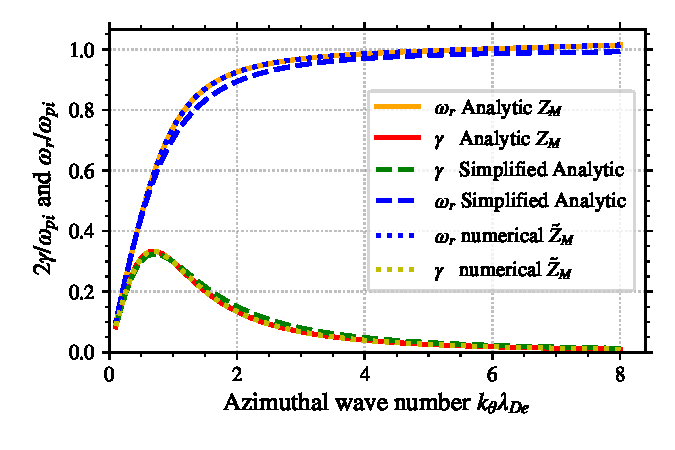
\includegraphics[width=\defaultwidth]{IAW_Maxw}
    \caption{IAW frequency and growth rate for a Maxwellian distribution function using the Freid and Conte function (labelled Analytic $Z_M$), the numerical estimation of $\tilde{Z}_M$, and the simplified analytic expressions of \cref{eq-MIAW}. }
    \label{fig-IAW_Maxw}
  \end{figure}
  
  We can see that all results gives almost the same solutions.
  The growth rates are all overlapping, hence it is difficult to see the differences.
  For $\omega_r$, the simplified analytic expression returns a slightly different result, but the differences is negligible.
  The numerical evaluation of $\tilde{Z}_M$ gives the same result as analytic evaluation.
  
  \Cref{fig-IAW_druv} shows the effect of a Druyvesteyn electron distribution compared to a Maxwellian.
  We recall that a Druyvesteyn distribution follows the expression
  \begin{equation} \label{eq-druyv}
    f_{D}(v) = \exp \lp C1 \frac{\norm{v}^3}{v_{th}^3}  \rp C2,
  \end{equation}
  with $C1 \simeq 0.63$ and $C2 \sim 0.84$ two normalizing constants.
  We can see that there is no much impact of the Druyvesteyn electron velocity distribution function on the electron, except that the maximum growth rate is sightly diminished.
  
  \begin{figure}[hbt]
    \centering
    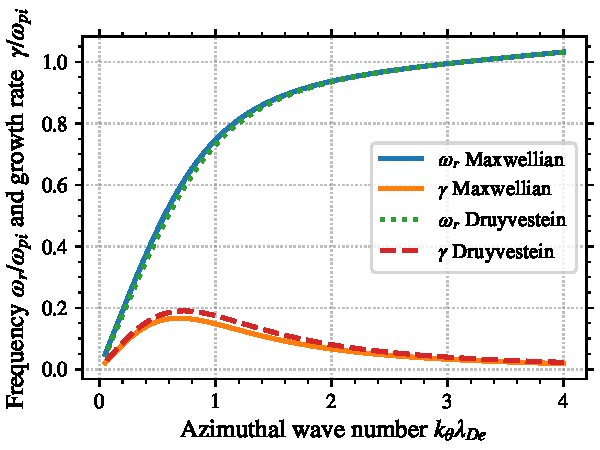
\includegraphics[width=\defaultwidth]{IAW_druv}
    \caption{IAW frequency and growth rate for a Maxwellian distribution function using the Freid and Conte function and a Druyvesteyn distribution evaluated with the numerical estimation of $\tilde{Z}$. }
    \label{fig-IAW_druv}
  \end{figure}
  
  \paragraph{Electron Cyclotron Drift instability\\}
  
    \Cref{fig-ECDI_druv} shows the frequency and the grow rate for the \ac{ECDI}, defined by \cref{eq-drECDI}, in the same conditions that the \ac{IAW} results, with $k_r \lambda_{De} = 0.1 $.
    The infinite sum over the cyclotron resonances is stopped at $N_{max} = 20$.
    
    
    \begin{figure}[hbt]
    \centering
    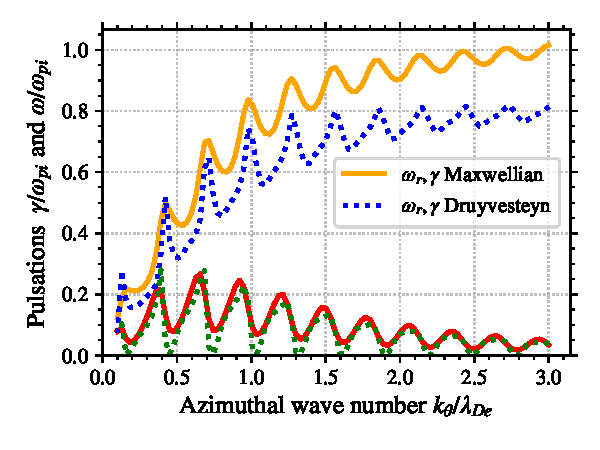
\includegraphics[width=\defaultwidth]{ECDI_druv}
    \caption{\acs{ECDI} frequency and growth rate for a Maxwellian distribution function using the Freid and Conte function and a Druyvesteyn distribution evaluated with the numerical estimation of $\tilde{Z}$, the radial wave number is $k_r \lambda_{De} = 0.1 $.}
    \label{fig-ECDI_druv}
  \end{figure}
  
  We can see in \cref{fig-ECDI_druv} that the cyclotron resonances are present for both distribution functions.
  But while the growth rate is not much affected, the frequency is reduced for the Druyvesteyn distribution for larger azimuthal wave number.
  
  For a smaller radial wavenumber, the numerical resolution crashes, as the argument in the $Z$ function diverges.
  However, in the limit $\eta \rightarrow \infty, Z(\eta) \rightarrow  \frac{1}{\eta}$.
  Hence, we still obtain the cyclotron resonances, as shown in \citet[Fig. 2]{janhunen2018}.
  
  
\let\rightmark=\oldrightmark

% !TEX root=/home/tavant/these/manuscript/src/manuscript.tex
\FloatBarrier
\section{Comparison of the \acs{DR} with the \acs{PIC} simulations}
  \label{sec-DR-results}
  
  

  \subsection{Temporal evolution of the distribution functions in the \acs{PIC} simulation} \label{subsec-VDFpic}
  
  To begging with, we visualize and comment the distribution functions measured in the \ac{PIC} simulation.
  \Cref{fig-vdfs_pic_time} shows at different moments in the simulation the ion and electron azimuthal velocity distribution functions, normalized.
  The velocities are normalized by the thermal speed of the respective species.
  To guide the reading of the figure, is added the  theoretical electron drift velocity $u_e = \frac{E_z}{B_r}$, normalized to the electron thermal speed, as well as the ion sound speed $c_s$, normalized to the ion thermal velocity.
  The distributions are averaged in time over $4\,\nano\second$, and in space over all the azimuthal direction.
  In the radial direction, the distributions are averaged over a small length at the center of the channel, between $r=0.45\,\centi\meter$ and $r=0.55\,\centi\meter$.
  
  \begin{figure}[!hbt]
    \centering
    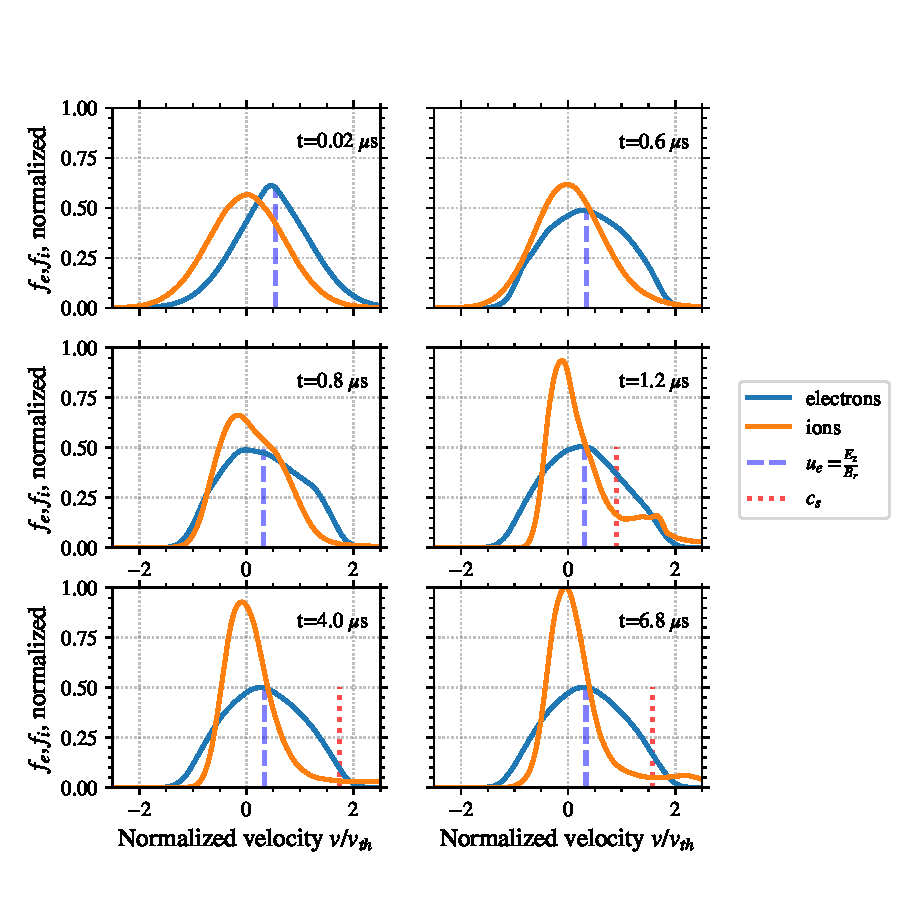
\includegraphics[width=0.95\textwidth]{Distributions_time_evolution_2.pdf}
    \caption{Electron and ion normalized azimuthal velocity distribution functions. The velocity in abscissa is normalized by the thermal speed of the corresponding species. Is overlaid the theoretical $E\times B$ drift velocity of the electrons $u_e = \frac{E_z}{B_r}$, and the ion sound speed $c_s$ normalized by the ion thermal velocity.}
    \label{fig-vdfs_pic_time}
  \end{figure}
  
  We can observe in \cref{fig-vdfs_pic_time} that the electron mean velocity is always the $E \times B$ drift velocity, which is of the order of one quarter of the electron thermal speed.
  On the other hand, at the beginning of the simulation the mean velocity of the ion is null.
  But we can see that starting from $t=.8\,\micro\second$, the ions are dragged in the same direction that the electron drift.
  This is characteristic of the ion-wave trapping \citep{lafleur2017a}
  Here, we have to be careful not to misread the figure.
  As we have $v_{th, e} > v_{th, i}$, the effective drift velocity of the ion is much less that the electron.
  % \inlinenote{Give the values here, like $ u_e, c_s, v_th$, etc. \\ Anne: oui pour mettre des valeurs}
  
  We can see that a small population of high energy ions is generated, because of particle-wave interactions.
  This leads to both an increase ion temperature, and the formation of a drift velocity in the azimuthal direction.
  The high energy ion population comes from ion trapping, as we can see that their velocity is of the order of the ion sound speed, which is close to the wave phase velocity \citep{lafleur2018}.
  
  As both electron and ion velocity distribution functions are far from a drifting Maxwellian, we will study the influence of both distributions in the calculations of the dispersion relation.
  
  
  % \FloatBarrier
  \subsection{Resolution of the electron cyclotron drift instability} \label{subsec-ECDIPIC}
  
  
    As observed in \Cref{sec-PIC-ECDI}, the simulation begins by a linear growth of the instability.
    Previous results obtained with \LPPic \citep{croes2017a} showed no resonances during this period.
    However, these results where obtained with Lafleur's convection model, as introduced in \cref{sec-reinjectionnoise}.
    Here, the results where obtained with the modified model, inducing less noise.
    The parameters used for the simulation are given in \cref{tab-evdfpicparams}.
    
    We can see in \Cref{fig-phi_fluctuation_summary}  a snapshot of the plasma potential fluctuation in the azimuthal direction \[ \delta \phi(r, \theta) = \phi(r, \theta) - < \phi(r, \theta) >_{ \theta}, \]
    at four different times during the growth of the instability.
    For these results, we increased the azimuthal length $L_{\theta}$ from $2.5$ to $6.2\,\milli\meter$ compared to the simulations of \cref{ch-2,sec-PIC-ECDI}, so that the instability characteristics, as the wavenumber $k$, are more distinguishable.
    We observe no significant differences on the simulation results.
    However, the simulation time is doubled in this case, so only the first microseconds have been simulated.
    

    
    \begin{figure}[!hbt]
      \centering
      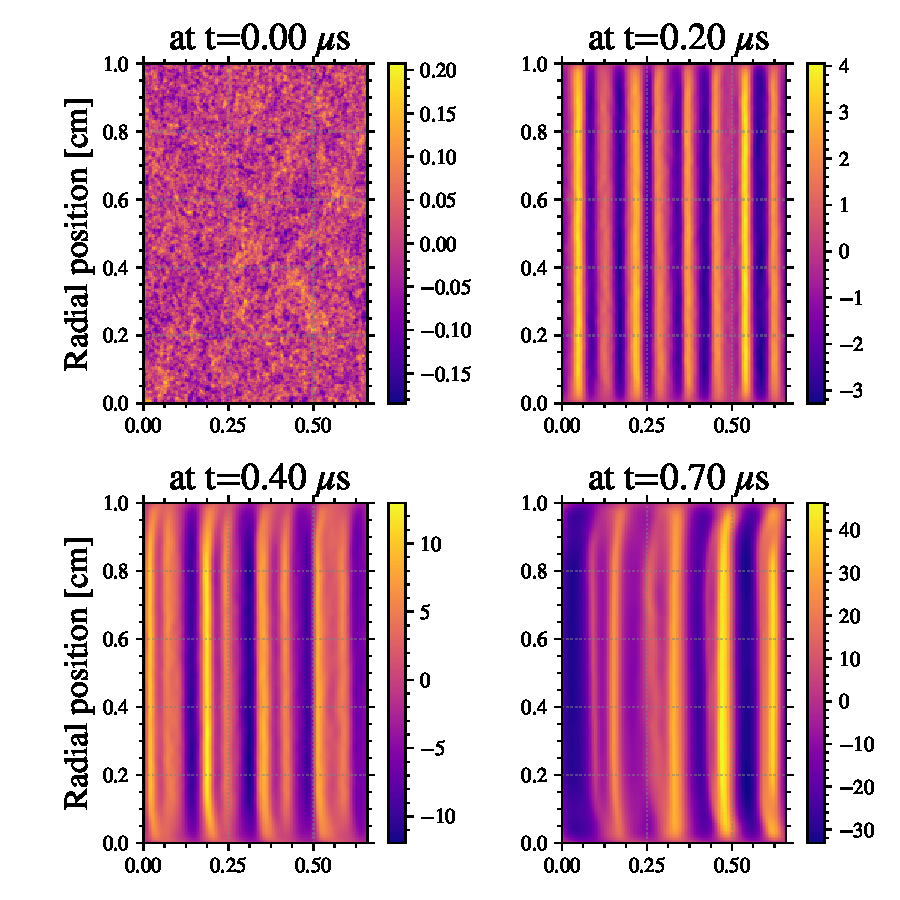
\includegraphics[width=0.8\textwidth]{phi_fluctuation_summary.pdf}
      \caption{Snapshot of the plasma potential at different times during the linear phase of the simulation. The frequency spectra of each snapshot is showen in \cref{fig-phi_fluctuation_summary_FFT}. }
      \label{fig-phi_fluctuation_summary}
    \end{figure}
    
    At the beginning, we see fluctuations that can be due to both thermal fluctuation \citep{salpeter1960} or numerical noise due to particle discretization.
    Then, the instability rises.
    We can see that it starts with small wavelength ($\lambda \simeq 0.75\,\milli\meter$ at $t=0.2\,\micro\second$).
    After a short period, the short wavelength waves merges to form longer wavelength waves  ($\lambda \simeq 1.5\,\milli\meter$ at $t=0.7\,\micro\second$).
    
    
    \begin{figure}[!hbt]
      \centering
      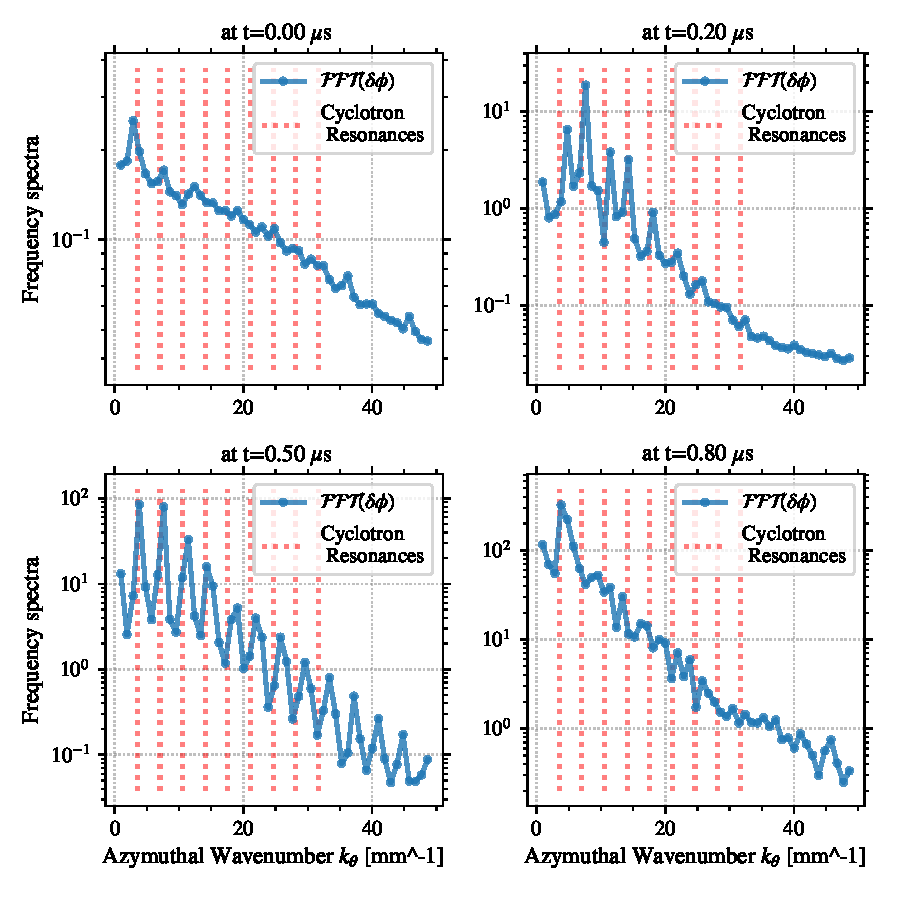
\includegraphics[width=0.8\textwidth]{phi_fluctuation_summary_FFT.pdf}
      \caption{Frequency spectra on the azimuthal instability presented in \cref{fig-phi_fluctuation_summary}. Each spectrum is averaged in the radial direction. The red dotted lines represent the cyclotron resonances.}
      \label{fig-phi_fluctuation_summary_FFT}
    \end{figure}
    
    This is also clearly seen on the frequency spectra, showed in \Cref{fig-phi_fluctuation_summary_FFT}.
    We can see in the spectra the resonances at the cyclotron wavenumber $k_0 = \frac{\oce}{u_e} \simeq 3.5\,\milli\meter^{-1}$.
    At $t=0.2\,\micro\second$, the most dominant mode is the second resonance, but the other resonances start to appear.
    At $t=0.4\,\micro\second$, all of the resonances are distinguishable, but their amplitude is strictly decreasing.
    Then, at $t=0.7\,\micro\second$, we can no longer see the resonances, except for the first one.
    As we observed during the first stages of the simulation the resonances in the Fourier spectrum, we solve the dispersion relation for the \ac{ECDI}.
    
    \vspace{1em}
    We solve the \ac{ECDI} dispersion relation of \cref{eq-drECDI} for $t=0.2, 0.4$ and $0.7\micro\second$ using both the Maxwellian hypothesis for the ions and electrons, and the velocity distribution functions measured in the \ac{PIC} simulations.
    The radial wavenumber taken is $k_r = 2 \pi/L_R \sim 0.6 \per\milli\meter$ \citep{lafleur2016,janhunen2018}.
    This value corresponds to $k_r \lde = 0.036$ at $t=0.2\,\micro\second$ and $k_r \lde = 0.044$ at $t=0.7\,\micro\second$, as the electron temperature increases.
    
    \begin{figure}[!hbt]
      \centering
      % \begin{tabular}{c}
        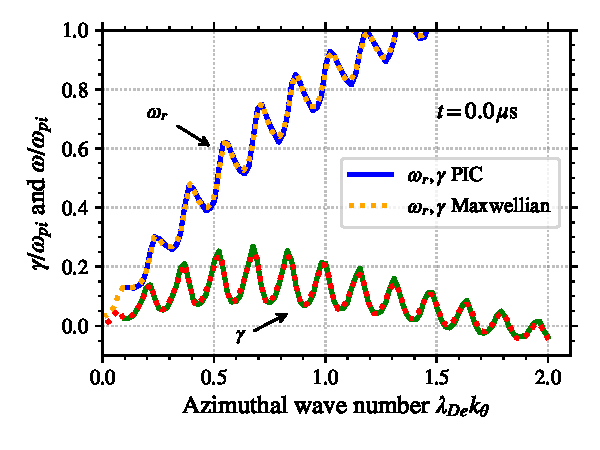
\includegraphics[width=0.49\textwidth]{ECDI_PIC_ionvcorrected_2mus.pdf} 
        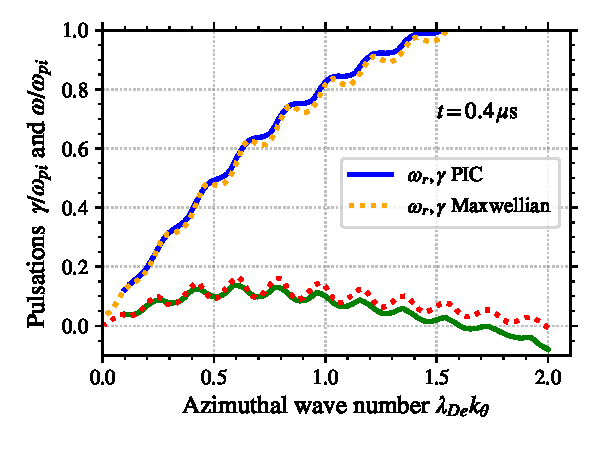
\includegraphics[width=0.49\textwidth]{ECDI_PIC_ionvcorrected_4mus.pdf} 
        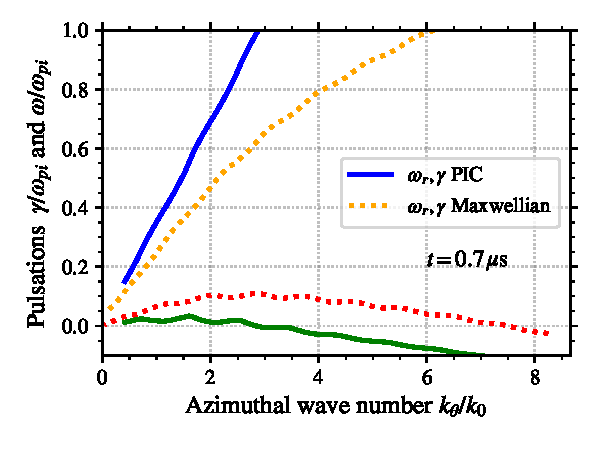
\includegraphics[width=0.49\textwidth]{ECDI_PIC_ionvcorrected_7mus.pdf} 
      % \end{tabular}
      \caption{Dispersion relation for the \acs{ECDI} using both (dotted lines) the Maxwellian hypothesis for the ions and electrons, and (solid lines) the velocity distribution functions measured in the \acs{PIC} simulations. The abscissa is normalized by the cyclotron resonance wavelength.}
      \label{fig-DRECDI}
    \end{figure}
    
    We can see in \Cref{fig-DRECDI} that the dispersion relation shows the cyclotron resonance at the beginning.
    However, the most growing wavelength is not the second harmonic, but the forth.
    After $t=0.4\,\micro\second$, the resonances broaden, and disappear.
    This is due to the increases of the radial wavelength used with respect to the Debye length $\lde$ \citep{lafleur2016a,ducrocq2006,cavalier2013}.
    The value of radial wavelength is discuss later in \cref{sec-DR-BC}.
    
    We can also observe that the deviation of the distribution function from the Maxwellian decreases the growth rate.
    This has been observed  in an axial-azimuthal \ac{PIC} simulation by \citet{lafleur2018}.
    This confirms that the exact distribution function should be used in the calculation of the dispersion relation, especially to determine the growth rate.
    \Cref{fig-DR_and_fft} shows a comparison of the \ac{2D} \ac{FFT} of the azimuthal electric field FFT$(E_{\theta})$ computed between  $t=0.6\,\micro\second$ and $t=1.2\,\micro\second$  with the three dispersion relations\string:
    \begin{itemize}
      \item the \ac{ECDI} general \ac{DR} obtained with the \ac{PIC} \ac{EVDF} at $t=0.6\,\micro\second$,
      \item the \ac{ECDI} \ac{DR} obtained with the Maxwellian hypothesis,
      \item the \ac{IAW} \ac{DR} using the analytic expression \cref{eq-MIAW}. 
    \end{itemize}
    The two first \ac{DR} are already showed in \cref{fig-DRECDI} with there corresponding growth rates.

    \begin{figure}[!hbt]
      \centering
      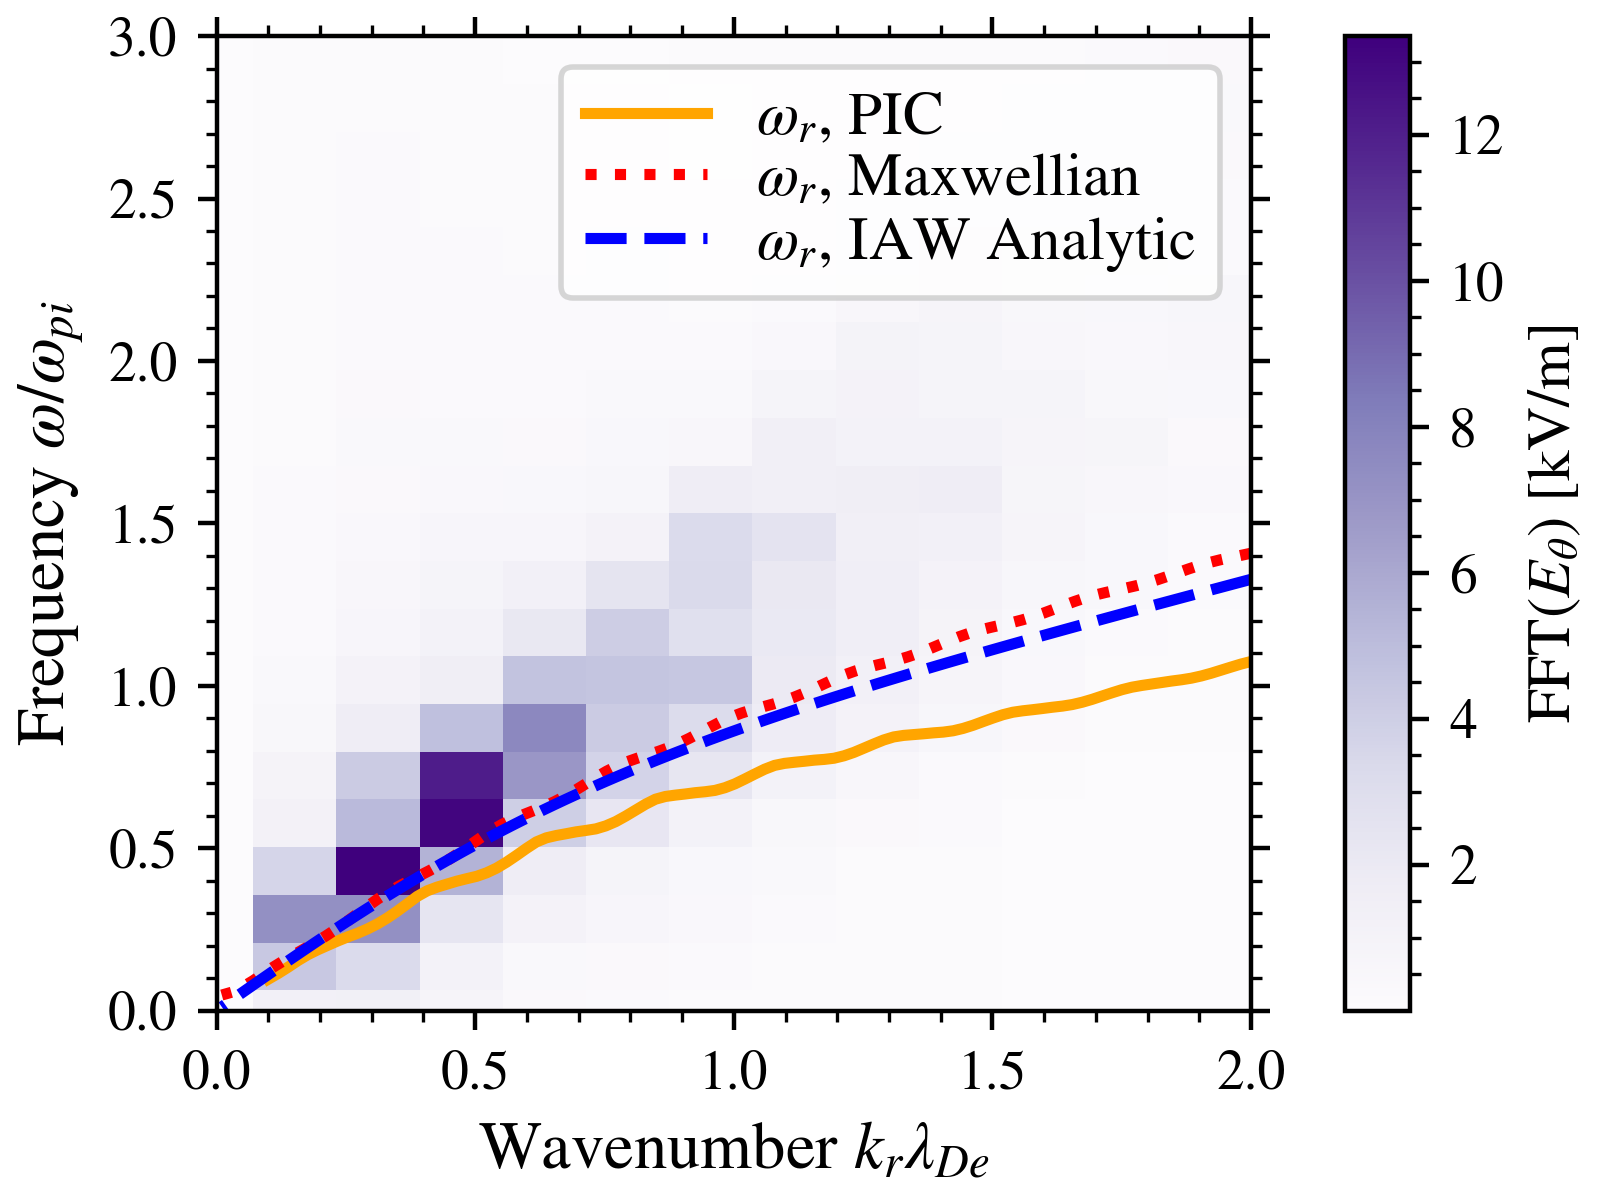
\includegraphics[width=\defaultwidth]{compe_fft_theo}
      \caption{Comparison of the \acs{2D} \acs{FFT} of the azimuthal electric field FFT$(E_{\theta})$ with the following \acs{DR}\string: (orange solid) \acs{ECDI} general \acs{DR} obtained with the \acs{PIC} \acs{EVDF}; (dotted red) \acs{ECDI} \acs{DR} obtained with the Maxwellian hypothesis; and (dotted blue) \acs{IAW} \acs{DR} using the analytic expression \cref{eq-MIAW}.   }
      \label{fig-DR_and_fft}
    \end{figure}
    
    From \Cref{fig-DR_and_fft}, we can see that the \ac{PIC} result does follow the \ac{ECDI} \ac{DR} with a very good correspondence.
    However, the differences between the three \ac{DR} are not significant, compared to the resolution of the \ac{2D} \ac{FFT}.
    On top of that, the \ac{IAW} \ac{DR} returns almost the same values than the \ac{ECDI} \ac{DR}, as the resonances are no more present.
    
  \FloatBarrier
  \subsection{Resolution of the ion acoustic wave dispersion relation} \label{subsec-VDFIAW}
  
  We have seen in the previous \cref{subsec-ECDIPIC} that the full \ac{ECDI} dispersion relation is not needed, but can instead be approximated by the \ac{IAW} \citep{lafleur2018,janhunen2018,taccogna2019}.
  The \ac{IAW} relation can be solved with several hypotheses (see \cref{sec-geneDR} for more details)
  \begin{enumerate}
    \item Simplified analytical values,
    \item Maxwellian electrons, cold ion ($\Ti = 0\,\volt$),
    \item Maxwellian electrons and ions ($\Ti > 0\,\volt$),
    \item Non-Maxwellian electrons, Maxwellian ions ($\Ti > 0\,\volt$),
    \item Non-Maxwellian electrons and ions.
  \end{enumerate}
  
  We will use all of these cases, and compare them to the \ac{PIC} simulation results.
  We want to obtain the temporal evolution of the solution.
  In practice, we will only follow the evolution of the most growing wave.
  In order to find the most growing wave, we solve the dispersion relation for different values of $k$.
  Over all of the solutions obtained, we select the one corresponding to the maximum value of $\gamma$.
  We use 100 values between $k=0.02 \lde$ and $k = 2 \lde$.
  \Cref{fig-Example_of_DR_IAW} illustrates the protocol used for 3 different cases.
  We can see the maximum of the growing rate, and its frequency.
  
  \begin{figure}[hbt]
    \centering
    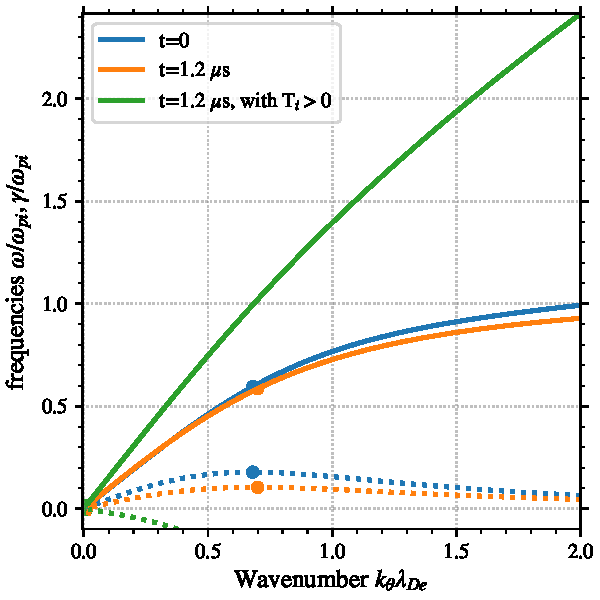
\includegraphics[width=4.5in]{Example_of_DR_IAW.pdf}
    \caption{Illustration of the \acs{IAW} dispersion relation obtained at two different time ($t=0$ and $t=1.2\,\micro\second$), (solid line) the wave frequency $\omega$, and (dotted line) the growth rate $\gamma$, using the hypothesis of Maxwellian distribution functions for both electrons and ions. The electron temperature measured in the simulation is always used, but the ion temperature is only used once. The most growing solution is marked with a circle on the growing rate and the frequency.}
    \label{fig-Example_of_DR_IAW}
  \end{figure}
  
  
  This calculation is automated for the whole duration of the simulation.
  The velocity distribution functions, when used, are obtained from the \ac{PIC} simulation the same way that in \cref{subsec-VDFpic}.
  \Cref{fig-time_wave} shows the temporal evolution of the three characteristics of the most growing wave: the growth rate $\gamma$, the azimuthal wavenumber $k$ and the frequency $\omega$.
  \begin{figure}[hbt]
    \centering
    % 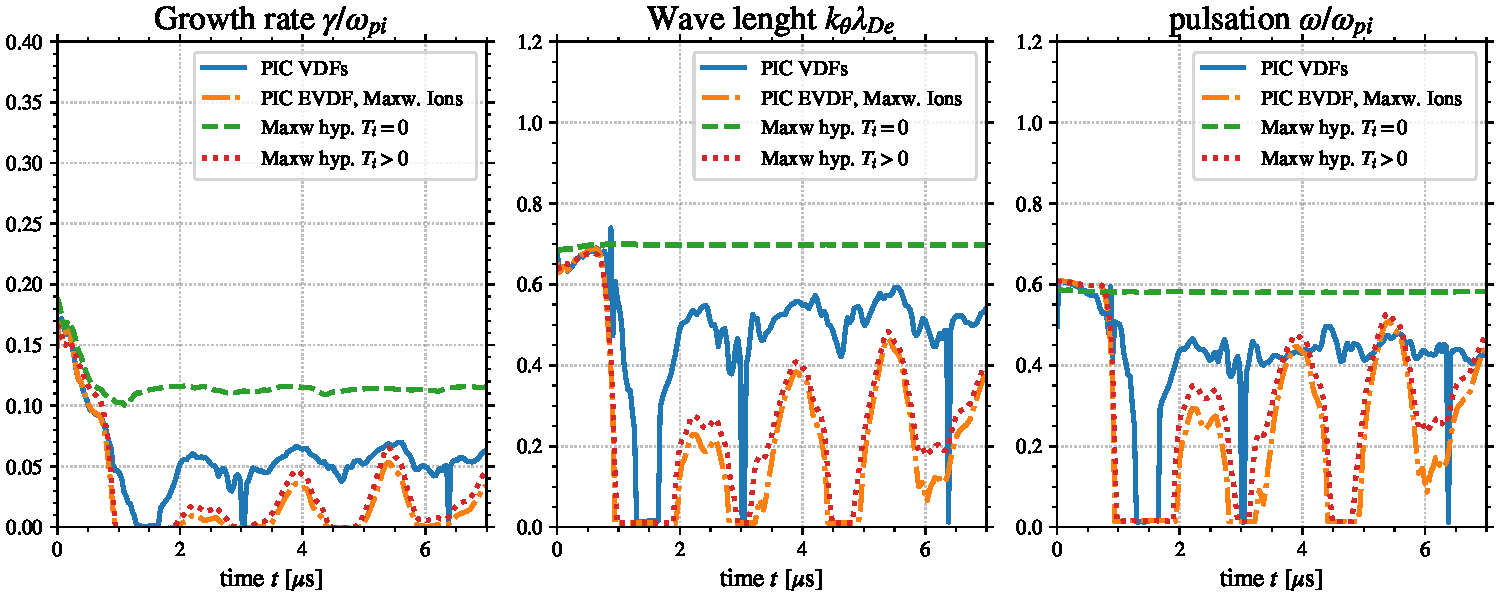
\includegraphics[width=\textwidth]{GrowthRate_time_evolution_250_ter.pdf}
    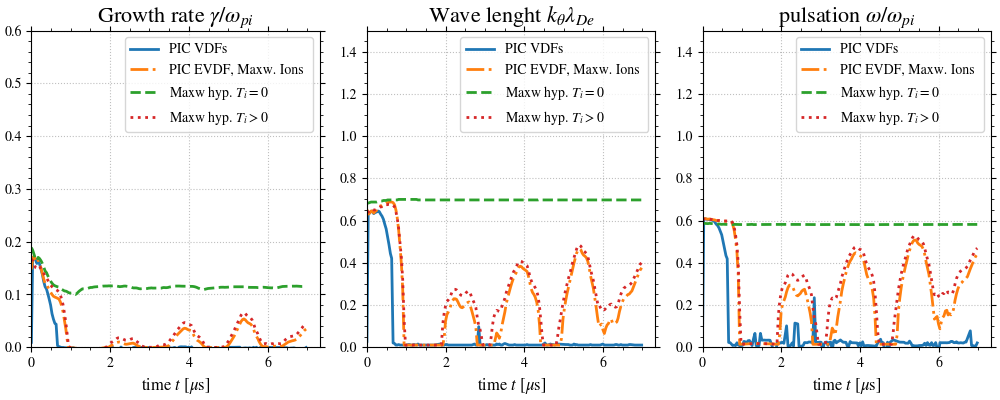
\includegraphics[width=\textwidth]{GrowthRate_time_evolution_250_again.png}  %inverted ion velocity as a correction, to look like Lefleur... :/
    \caption{Temporal evolution of the growth rate $\gamma$, the azimuthal wavenumber $k$ and the frequency $\omega$ for the most growing wave, obtained with several hypotheses on the dispersion relation. See text for more precisions. }
    \label{fig-time_wave}
  \end{figure}
  
  Three different behaviors are observed depending on the hypotheses used.
  First, the solution of the dispersion relation with Maxwellian electrons and cold ions (dashed green line in \cref{fig-time_wave}) presents a solution of $\omega$ and $k$ constant in time, and very close to the analytical values, beeing $k \lde = 1/\sqrt{2}$ and $\omega = \opi/\sqrt{3}$.
  However, it also presents a constant growth rate.
  Secondly, we observe that the solutions given with Maxwellian ions of temperature not zero are relatively similar for both the Maxwellian electrons  (dotted red line) and using the electron velocity distribution function measured in the \ac{PIC} simulation (dash-dotted orange line).
  In these cases, the growth rate decreases regularly to zero.
  
  Interestingly, the periods during which the growth rate is zero (firstly between $t=1\,\micro\second$ and $t=2\,\micro\second$, then around $t=3\,\micro\second$ and so on) correspond precisely to the periods during which the wave energy density decreases in \cref{fig-tempITcrit}.
  This means that the decrease of the wave amplitude would only be due to the ion temperature, and not its distribution function.
  However, we note that the value of the ion temperature $\Ti$ is highly affected by the population of ions trapped, as seen in \cref{subsec-VDFpic}.
  Hence, the effect of the trapped particle is indeed present, but only via its impact on the temperature.
  
  \vspace{1em}
  To finish with, we solved the \ac{IAW} dispersion relation without any hypothesis on the velocity distribution functions, by using the one measured in the PIC simulations (blue solid line in  \cref{fig-time_wave}).
  In this case, the beginning ($t < 1 \,\micro\second$) is quite similar to the other results.
  However, after that ($t > 1 \,\micro\second$) the growth rate never rises above zero, expect very slightly around $t=4\,\micro\second$.
  This result is non consistent with the observations of \cref{sec-PIC-ECDI}, where we saw that the instability amplitude is modulated over the whole simulation time.
  It is also in contrast with \citet{lafleur2018}, where the authors obtained a non-zero growth rate in an axial- azimuthal geometry.
  
  Up to now, there is non apparent explanation to the dependency  observed between the numerical resolution of the \ac{DR} and the results of the \ac{PIC} simulation.
  It could be due to an error in the numerical algorithm, on both on the theory and in the implementation.
  Concerning the theory, we have seen in \cref{sec-DR-solver} that the numerical algorithm used to compute the plasma dispersion function $\tilde{Z}$ proposed by \citet{xie2013} does not return a good result for certain argument complex values.
  In addition, the truncation of the number of Fourier bases at $N=64$, which works well with a Maxwellian distribution, could generate a significant error when using distribution function far from a Maxwellian.
  In our specific case, the ion population is composed of a majority of cold Maxwellian ions and a small number of high energetic trapped ions.
  It is possible that this kind of distribution function is not well taken into account by the current algorithm.
  
  Concerning the implementation of the algorithm, we tried to test and validate the code as much as we can, with systematic comparaisons to analytic values.
  But the presence of an error is always possible, that was not observed on the analytic functions.
  A common practice to validate a simulation code when no theoretical solution can be used to compare to is to use a Benchmark \citep{turner2013}.
  As a dispersion relation solver for general distributions would benefit the whole plasma physics community, developing such a benchmark that would compare the solution of independent implementations of the same algorithm, or different algorithm, seems very interesting.
  
  \FloatBarrier
% !TEX root=/home/tavant/these/manuscript/src/manuscript.tex

\section{ Discussion on the radial wavenumber}
  \label{sec-DR-BC}
    
  In the \ac{ECDI} dispersion relation described in \cref{sec-DR-kinetic}, the radial wavenumber must be non-zero.
  Hence, in \cref{sec-DR-results}, we have chosen a wavelength that fits between the two walls.
  On the other hand, the oscillation seen in \cref{fig-phi_fluctuation_summary} seems not to present any oscillation in the radial direction.
  In this section, we investigate the interaction between the azimuthal instability and the wall in the radial direction.
  
  \subsection{Radial profile of the oscillation} \label{subsec-radial_prof}
  \Cref{fig-phi_osci_profile} shows the amplitude of the azimuthal instability on the plasma potential.
  It is defined as
  \begin{equation} \label{eq-stdphi}
    \delta \phi^2 = 2 \sigma_{\phi}^2 = \frac{{2}}{L_{\theta}} \int_0^{L_{\theta}} \lp  \phi - <\phi>_{\theta}  \rp ^2 d\theta,
  \end{equation}
  
  \begin{figure}[hbt]
    \centering
    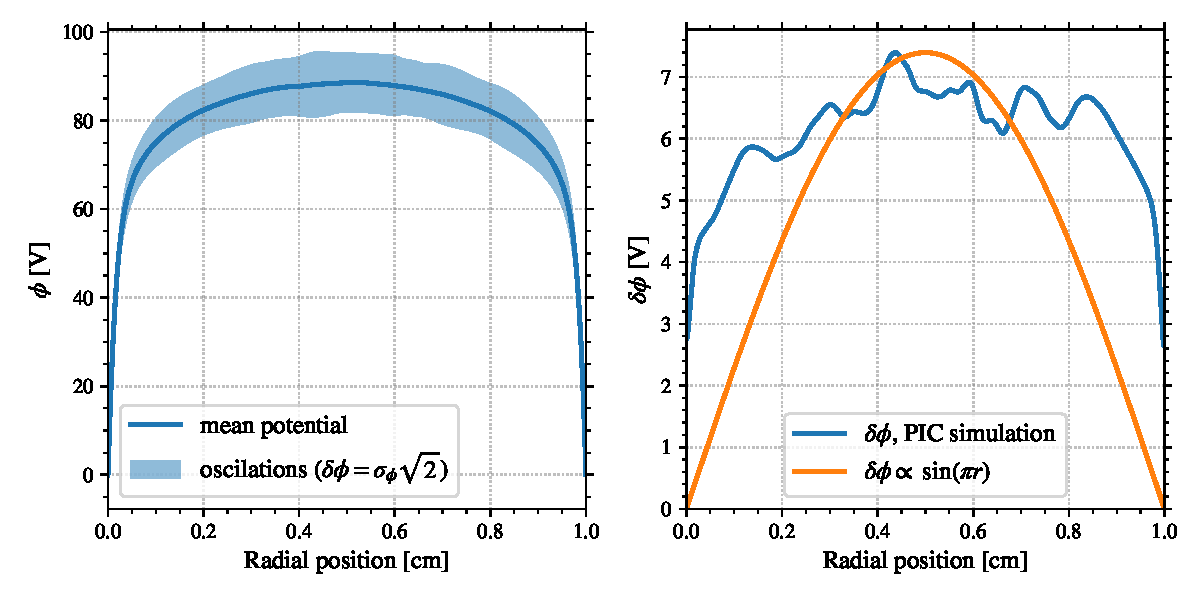
\includegraphics[width=\textwidth]{phi_oscillation}
    \caption{(Left) Radial profile of the mean plasma potential averaged in the azimuthal direction  and in time during the steady-state of the simulation ($t > 3.5 \,\micro\second$) and the average azimuthal instability amplitude. (Right) Radial profile of the  azimuthal instability amplitude, compared with a sinusoidal profile. }
    \label{fig-phi_osci_profile}
  \end{figure}
  
  
  We see in \cref{fig-phi_osci_profile} that the amplitude of the oscillation in the radial direction does not follow a sinusoidal profile, that would be the characteristic of a non-zero radial wavenumber.
  This observation contradicts the hypothesis made previously on the value of $k_r$.
  In order to better apprehend the radial profile of the instability amplitude, we study the ratio between $\delta \phi$ the fluctuation amplitude (showed on the right in \cref{fig-phi_osci_profile}) and $<\phi>_{\theta}$  the mean plasma potential (on the left in \cref{fig-phi_osci_profile}).
  
  \begin{figure}[hbt]
    \centering
    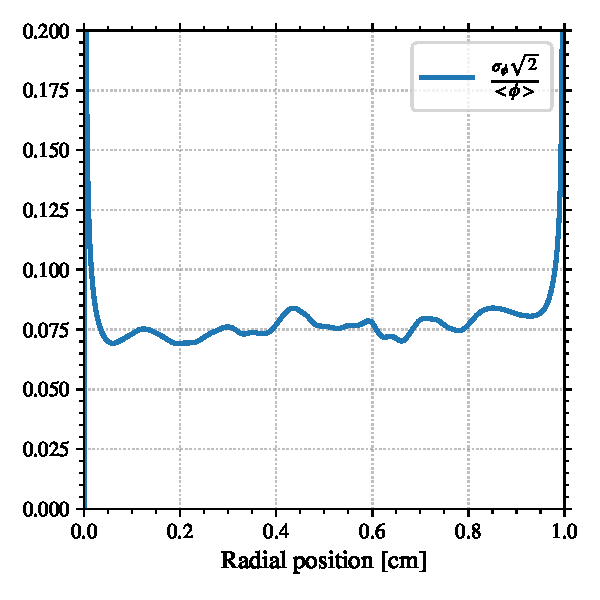
\includegraphics[width=\defaultwidth]{phi_oscillation_ratio}
    \caption{Radial profile of the ratio between $\delta \phi$ the fluctuation amplitude (showed on the right in \cref{fig-phi_osci_profile}) and $<\phi>_{\theta}$  the mean plasma potential (on the left in \cref{fig-phi_osci_profile}).}
    \label{fig-ratio}
  \end{figure}
  
  \Cref{fig-ratio} shows that the ration $\frac{\delta \phi}{ <\phi>_{\theta}}$ is almost constant in the plasma, except close to the wall, where the plasma potential decreases much faster than the oscillations.
  The same behavior  observed in the profiles of the ion density, that can be seen in \Cref{fig-ion_oscilation}.
  As a mater of fact, the behavior even more pronounced on the ion density, as the ratio $\delta n_i / n_i$ presents a radial profile almost constant.
  It can be explains by the fact the ions reaches the wall with an supersonic speed, so that the wall does not directly affected the ions.
  
  
  \begin{figure}[hbt]
    \centering
    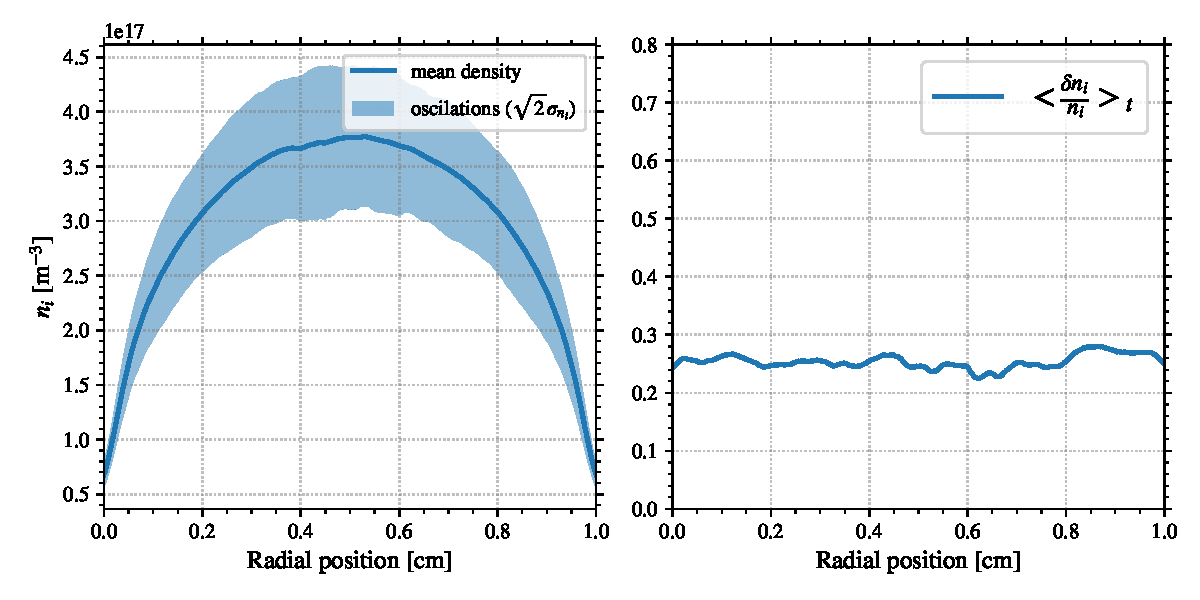
\includegraphics[width=\textwidth]{Ion_oscilations.pdf}
    \caption{Radial profile of (left) the mean ion density profile and $\delta n_i$ the fluctuation amplitude and (right) the ratio between $\delta n_i$ and $n_i$.}
    \label{fig-ion_oscilation}
  \end{figure}
  
  \vspace{1em}
  This may suggest that the sheaths screen  the walls significantly from the oscillations,  which are therefore not affected.
  A screening of the wall have been observed in \citet{janhunen2018}, where the authors observed radial structures of wavelength larger than the radial length.
  However, here we observe no radial structure.
  The difference between  \citet{janhunen2018} and the results presented here may be due to the difference in the radial length ($L_R =1 \,\centi\meter$ here, against $L_R = 5.38\,\centi\meter$).
  
  \subsection{Impact of the radial wavenumber on the \acs{DR}}
   \label{subsec-kr}

  To highlight the impact of the radial wavenumber on the \ac{ECDI} \ac{DR}, \cref{fig-kreffect} shows for three values of $k_r \lde$ the evolution of the frequency $\omega$, and  the growth rate $\gamma$ as a function of the azimuthal wavenumber $k_{\theta}$.
  We see that when $k_r \lde$ increases from 0.02 to 0.1, the cyclotron resonances decrease and broaden until they disappear.
  \begin{figure}[!hbt]
    \centering
    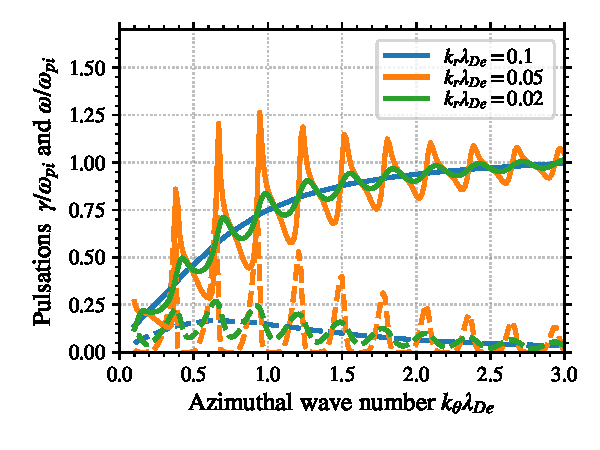
\includegraphics[width=\defaultwidth]{ECDI_ktheta_impact.pdf}
    \caption{Evolution as a function of the azimuthal wavenumber $k_{\theta}$ of (solid line) the frequency $\omega$, and (dashed line) the growth rate $\gamma$ for three values of the normalized radial wavenumber $k_r \lde$. }
    \label{fig-kreffect}
  \end{figure}
  
  This reduction of the resonances explains the observations of \cref{fig-DRECDI}, where we saw similar reduction of the cyclotron resonances, due to the increase of $\lde$ the Debye length from $\lde=\sn{4.3}{-5}\,\meter$ at $t=0$ to $\lde=\sn{7.0}{-5}\,\meter$ at saturation.
  However, if the radial wavenumber $k_r$ tends toward zero, in agreement with the observations of \cref{fig-ion_oscilation}, then the resonances would not smooth out for this reason.
  Instead, the resonances would stay.
  
  \vspace{1em}
  As a conclusion, the interaction between the instability and the boundaries is not clearly understood.
  The sheaths seem to  screen the waves from the radial boundaries.
  In \Cref{subsec-BC}, we will discuss on the impact of the radial boundary condition (metallic versus dielectric electrode) on the oscillation, but the conclusion will be similar.

  As there is no radial structure observed in the simulation showed here, it means that the oscillation is purely azimuthal, or at least $\lde k_r <<1$.
  In this case, the cyclotron resonances should non-longer disappear \citep{ducrocq2006}, except due to non-linear demagnetization of the electrons, as discussed before \citep{boeuf2018,taccogna2019}.
  The non-linear dispersion relations are out of the scope of the present work, but should be developed in order to better understand the evolution on the \ac{ECDI} in the \ac{HET}.
  
  To understand the divergent observations of \citet{hara2019a,janhunen2018,taccogna2019}, a comparisons of the simulation results using similar parameter and models should be undertaken.
  Such a comparison is currently undertook between the different working groups on another simulation case. 
  Once this first Benchmark is conducted, the radial-azimuthal geometry should be studied.
  
  
  
  
